\chapter{Arhitektura i dizajn sustava}
		
		%\textbf{\textit{dio 1. revizije}}\\

		%\textit{ Potrebno je opisati stil arhitekture te identificirati: podsustave, preslikavanje na radnu platformu, spremišta podataka, mrežne protokole, globalni upravljački tok i sklopovsko-programske zahtjeve. Po točkama razraditi i popratiti odgovarajućim skicama:}
	%\begin{itemize}
		%\item 	\textit{izbor arhitekture temeljem principa oblikovanja pokazanih na predavanjima (objasniti zašto ste baš odabrali takvu arhitekturu)}
		%\item 	\textit{organizaciju sustava s najviše razine apstrakcije (npr. klijent-poslužitelj, baza podataka, datotečni sustav, grafičko sučelje)}
		%\item 	\textit{organizaciju aplikacije (npr. slojevi frontend i backend, MVC arhitektura) }		
	%\end{itemize}

	\noindent{Arhitektura se dijeli na tri podsustava:}
	\begin{packed_item}
		\item web poslužitelj
		\item web aplikaciju
		\item bazu podataka
	\end{packed_item}
	\noindent{Web aplikacije često zahtijevaju integraciju poslužitelja, aplikacije i baze podataka kako bi pružile korisnicima dinamičke i interaktivne sadržaje. \textbf{Web poslužitelj} služi kao središnja točka koja prima zahtjeve korisnika putem internetskog preglednika. \textbf{Web aplikacija} obrađuje zahtjev te ovisno o njemu komunicira s bazom podataka kako bi dohvatila, mijenjala ili pohranjivala podatke koji se koriste u procesu. \textbf{Baza podataka} je skup strukturiranih podataka koji se čuvaju na poslužitelju, a aplikacija je odgovorna za upravljanje tim podacima i osiguravanje njihove konzistentnosti. Kada se podaci mijenjaju putem aplikacije, te promjene se ažuriraju u bazi podataka, a zatim web poslužitelj šalje ažurirane informacije korisnicima putem preglednika.}
	\newline
	\noindent{Jezici korišteni pri izradi aplikacije su C\#, CSS, HTML i JavaScript.}
	\newline
	\noindent{Arhitektura sustava se bazira na \textbf{MVC} konceptu. MVC (Model-View-Controller) je arhitekturni obrazac za razvoj softverskih aplikacija. \textbf{Model} predstavlja podatke i logiku aplikacije, \textbf{View} predstavlja sučelje preko kojeg korisnici komuniciraju s aplikacijom i prikazuje im podatke iz Modela, dok \textbf{Controller} upravlja komunikacijom između Modela i View-a. Ovaj koncept omogućava jasnu organizaciju koda, razdvajanje odgovornosti između komponenti aplikacije (Model, View, Controller) te olakšava timsku suradnju i održavanje aplikacije. Zbog jasne podjele na modele, poglede i kontrolere, aplikacije izgrađene na MVC arhitekturi često su fleksibilnije i lakše za održavanje.}

	\pagebreak
				
		\section{Baza podataka}
			
			%\textbf{\textit{dio 1. revizije}}\\
			
		%\textit{Potrebno je opisati koju vrstu i implementaciju baze podataka ste odabrali, glavne komponente od kojih se sastoji i slično.}
		Za pohranu podataka iz naše web aplikacije napravljena je relacijska baza podataka. Tablicama i njihovim atributima ostvarena je komunikacija između organiziranosti, preciznosti i jednostavnog dohvaćanja podataka za daljnu obradu. Baza podataka je kreirana u SQLite-u, upravo zbog toga što se podaci iz baze mogu dijeliti između više računala i jer koristi jednu datoteku za pohranu cijele baze podataka.\\
		Baza podataka se sastoji od sljedećih entiteta:
		\begin{packed_item}
			\item User
			\item Regular
			\item Shelter
			\item TypeOfUser
			\item Communication
			\item Ad
			\item PhotoAd
			\item Pet
			\item ColorPet
			\item hasColor
		\end{packed_item}
		
			\subsection{Opis tablica}
			

				%\textit{Svaku tablicu je potrebno opisati po zadanom predlošku. Lijevo se nalazi točno ime varijable u bazi podataka, u sredini se nalazi tip podataka, a desno se nalazi opis varijable. Svjetlozelenom bojom označite primarni ključ. Svjetlo plavom označite strani ključ}
				\textbf{Korisnik (User)}
				Ovaj entitet sadržava sve primarne informacije o korisniku. Sadrži atribute: userID, userName, email, phoneNum i psw. Ovaj entitet u vezi je \textit{One-to-Many} s entitetom Ad (oglas), \textit{One-to-Many} s entitetom Communication (Komunikacija) oba preko atributa userID korisnika te u vezi \textit{One-to-One} s entitetom Regular (redovni korisnik), \textit{One-to-One} s Shelter(sklonište) i \textit{One-to-One} s TypeOfUser (tip korisnika) preko userID - korisničkog imena.
				
				
				\begin{longtblr}[
					label=none,
					entry=none
					]{
						width = \textwidth,
						colspec={|X[6,l]|X[6, l]|X[20, l]|}, 
						rowhead = 1,
					} %definicija širine tablice, širine stupaca, poravnanje i broja redaka naslova tablice
					\hline \SetCell[c=3]{c}{\textbf{User}}	 \\ \hline[3pt]
					\SetCell{LightGreen} userID & INTEGER	& jedinstveni identifikator korisnika	\\ \hline
					userName & VARCHAR & naziv korisnika u aplikaciji \\ \hline 
					email & VARCHAR & e-mail adresa korisnika\\ \hline 
					phoneNum & VARCHAR	&  broj telefona korisnika\\ \hline
					psw & VARCHAR & lozinka korisnika\\ \hline
					%\SetCell{LightBlue} primjer	& VARCHAR &   	\\ \hline 
				\end{longtblr}
				
				\textbf{Redovni korisnik (Regular)}
				Ovaj entitet sadržava informacije o regularnom korisniku. Sadrži atribute: userID, firstName - ime i lastName - prezime korisnika. Ovaj entitet u vezi je \textit{One-to-One} s entitetom User (Korisnik) preko userID korisnika.
				
				
				\begin{longtblr}[
					label=none,
					entry=none
					]{
						width = \textwidth,
						colspec={|X[6,l]|X[6, l]|X[20, l]|}, 
						rowhead = 1,
					} %definicija širine tablice, širine stupaca, poravnanje i broja redaka naslova tablice
					\hline \SetCell[c=3]{c}{\textbf{Regular}}	 \\ \hline[3pt]
					\SetCell{LightBlue} userID & INTEGER	& jedinstveni identifikator korisnika, (user.userID)	\\ \hline
					firstName & VARCHAR & ime korisnika \\ \hline 
					lastName & VARCHAR & prezime korisnika\\ \hline 
					%\SetCell{LightBlue} primjer	& VARCHAR &   	\\ \hline 
				\end{longtblr}
				
				\textbf{Sklonište (Shelter)}
				Ovaj entitet sadržava informacije o skloništu kao korisniku. Sadrži atribute: userID i nameShelter - naziv skloništa. Ovaj entitet u vezi je \textit{One-to-One} s entitetom User (Korisnik) preko userID korisnika.
				
				
				\begin{longtblr}[
					label=none,
					entry=none
					]{
						width = \textwidth,
						colspec={|X[6,l]|X[6, l]|X[20, l]|}, 
						rowhead = 1,
					} %definicija širine tablice, širine stupaca, poravnanje i broja redaka naslova tablice
					\hline \SetCell[c=3]{c}{\textbf{Shelter}}	 \\ \hline[3pt]
					\SetCell{LightBlue} userID & INTEGER	& jedinstveni identifikator korisnika, (user.userID)	\\ \hline
					nameShelter & VARCHAR & naziv skloništa za životinje \\ \hline 
					
				\end{longtblr}
				
				\textbf{Tip korisnika (TypeOfUser)}
				Ovaj entitet sadržava informacije o tipu korisnika. Korisnik može biti regular - uobičajen korisnik ili shelter - sklonište za životinje. Sadrži atribute: userID i userType - tip korisnika. Ovaj entitet u vezi je \textit{One-to-One} s entitetom User (Korisnik) preko userID korisnika.
				
				
				\begin{longtblr}[
					label=none,
					entry=none
					]{
						width = \textwidth,
						colspec={|X[6,l]|X[6, l]|X[20, l]|}, 
						rowhead = 1,
					} %definicija širine tablice, širine stupaca, poravnanje i broja redaka naslova tablice
					\hline \SetCell[c=3]{c}{\textbf{TypeOfUser}}	 \\ \hline[3pt]
					\SetCell{LightBlue} userID & INTEGER	& jedinstveni identifikator korisnika, (user.userID)	\\ \hline
					userType & VARCHAR & tip korisnika - može biti shelter ili regular \\ \hline 
					 
				\end{longtblr}
				
				\textbf{Komunikacija (Communication)}
				Ovaj entitet sadržava sve važne informacije o komunikaciji ispod aktivnog oglasa. Sadrži atribute: textID, textCom - poruka, locCom - lokacija poruke te photoCom - slika unutar poruke te adID i userID - strani ključevi tablice Ad i User. Ovaj entitet u vezi je \textit{Many-to-One} s entitetom Ad (oglas) preko atributa adID oglasa i \textit{Many-to-One} s User preko userID korisnika.
				
				
				\begin{longtblr}[
					label=none,
					entry=none
					]{
						width = \textwidth,
						colspec={|X[6,l]|X[6, l]|X[20, l]|}, 
						rowhead = 1,
					} %definicija širine tablice, širine stupaca, poravnanje i broja redaka naslova tablice
					\hline \SetCell[c=3]{c}{\textbf{Communication}}	 \\ \hline[3pt]
					\SetCell{LightGreen} textID & INTEGER & jedinstveni identifikator poruke	\\ \hline
					photoCom & VARCHAR & slika poruke\\ \hline 
					textCom & VARCHAR & tekst poruke\\ \hline 
					locCom & VARCHAR	&  lokacija poruke\\ \hline
					\SetCell{LightBlue} adID	& INTEGER &  jedinstveni identifikator oglasa, (ad.adID)	\\ \hline 
					\SetCell{LightBlue} userID	& INTEGER & jedinstveni identifikator korisnika, (user.userID) 	\\ \hline
				\end{longtblr}
				
				\textbf{Oglas (Ad)}
				Ovaj entitet sadržava sve važne informacije o postavljanju oglasa. Sadrži atribute: adID, catID - kategorija oglasa, userID - strani ključ tablice User. Ovaj entitet u vezi je \textit{Many-to-One} s entitetom User (korisnik) preko atributa userID korisnika, \textit{One-to-Many} s Communication (Komunikacija) preko atributa adID, \textit{One-to-Many} s PhotoAd (slike oglasa) preko adID,
				\textit{One-to-One} s entitetom Pet(Ljubimac) preko adID oglasa.
				
				
				\begin{longtblr}[
					label=none,
					entry=none
					]{
						width = \textwidth,
						colspec={|X[6,l]|X[6, l]|X[20, l]|}, 
						rowhead = 1,
					} %definicija širine tablice, širine stupaca, poravnanje i broja redaka naslova tablice
					\hline \SetCell[c=3]{c}{\textbf{Ad}}	 \\ \hline[3pt]
					\SetCell{LightGreen} adID & INTEGER	& jedinstveni identifikator oglasa	\\ \hline
					catAd & VARCHAR & kategorije oglasa \\ \hline 
					\SetCell{LightBlue} userID	& INTEGER & jedinstveni identifikator korisnika, (user.userID)    	\\ \hline 
				\end{longtblr}
				
				\textbf{Slike oglas (PhotoAd)}
				Ovaj entitet sadržava sve važne informacije o postavljanju slika ispod oglasa. Sadrži atribute: photoID, photo - fotografija izgubljenog ljubimca, userID - strani ključ tablice User. Ovaj entitet u vezi je \textit{Many-to-One} s entitetom Ad (Oglas) preko atributa adID. Uz to, dodano je i ograničenje na razini baze - trigger za postavljanje maksimalno 3 slika uz oglas.
				
				
				\begin{longtblr}[
					label=none,
					entry=none
					]{
						width = \textwidth,
						colspec={|X[6,l]|X[6, l]|X[20, l]|}, 
						rowhead = 1,
					} %definicija širine tablice, širine stupaca, poravnanje i broja redaka naslova tablice
					\hline \SetCell[c=3]{c}{\textbf{PhotoAd}}	 \\ \hline[3pt]
					\SetCell{LightGreen} photoID & INTEGER	& jedinstveni identifikator slike oglasa	\\ \hline
					photo & VARCHAR & fotografija ljubimca \\ \hline 
					\SetCell{LightBlue} adID	& INTEGER &  jedinstveni identifikator oglasa, (ad.adID) 	\\ \hline 
				\end{longtblr}
				
				\textbf{Ljubimac (Pet)}
				Ovaj entitet sadržava sve važne informacije o nestalom kućnom ljubimcu. Sadrži atribute: petID, namePet - ime ljubimca, dateHourMis - datum i sat nestanka, location - lokacija pri postavljanju oglasa, vrsta ljubimca species, starost age, tekstni opis description i strani ključ adID iz Ad. Ovaj entitet u vezi je \textit{One-to-One} s entitetom Ad (oglas) preko atributa adID, \textit{Many-to-Many} s ColorPet (Komunikacija) preko tablice Has.
				
				
				\begin{longtblr}[
					label=none,
					entry=none
					]{
						width = \textwidth,
						colspec={|X[6,l]|X[6, l]|X[20, l]|}, 
						rowhead = 1,
					} %definicija širine tablice, širine stupaca, poravnanje i broja redaka naslova tablice
					\hline \SetCell[c=3]{c}{\textbf{Pet}}	 \\ \hline[3pt]
					\SetCell{LightGreen} petID & INTEGER & jedinstveni identifikator ljubimca	\\ \hline
					namePet & VARCHAR & ime na koje se odaziva ljubimac \\ \hline 
					dateHourMis & DATETIME & datum i sat nestanka ljubimca\\ \hline 
					location & VARCHAR	&  geolokacija izgubljenog ljubimca\\ \hline
					species & VARCHAR & vrsta ljubimca\\ \hline
					age & VARCHAR & starost ljubimca\\ \hline
					description & VARCHAR & opis ljubimca\\ \hline
					\SetCell{LightBlue} adID	& INTEGER &  jedinstveni identifikator oglasa, (ad.adID) 	\\ \hline 
				\end{longtblr}
				
				\textbf{Boja ljubimca (ColorPet)}
				Ovaj entitet sadržava sve važne informacije o boji kućnog ljubimca. Sadrži atribute: colorID i boja ljubimca color. Ovaj entitet u vezi je \textit{Many-to-Many} s entitetom Pet(Ljubimac) preko tablice Has.
				
				
				\begin{longtblr}[
					label=none,
					entry=none
					]{
						width = \textwidth,
						colspec={|X[6,l]|X[6, l]|X[20, l]|}, 
						rowhead = 1,
					} %definicija širine tablice, širine stupaca, poravnanje i broja redaka naslova tablice
					\hline \SetCell[c=3]{c}{\textbf{ColorPet}}	 \\ \hline[3pt]
					\SetCell{LightGreen} colorID & INTEGER	& jedinstveni identifikator boje ljubimca	\\ \hline
					color & VARCHAR & boja ljubimca \\ \hline 
					
				\end{longtblr}
				
				\textbf{ImaBoju (Has)}
				Ovaj entitet spaja boju i kućnog ljubimca. Sadrži atribute jedinstvene šifre colorID i petID. Ovaj entitet u vezi je \textit{Many-to-Many} s entitetom Pet(Ljubimac) preko atributa petID te u vezi \textit{Many-to-Many} s entitetom ColorPet(boja ljubimca) preko atributa colorID.
				
				
				
				\begin{longtblr}[
					label=none,
					entry=none
					]{
						width = \textwidth,
						colspec={|X[6,l]|X[6, l]|X[20, l]|}, 
						rowhead = 1,
					} %definicija širine tablice, širine stupaca, poravnanje i broja redaka naslova tablice
					\hline \SetCell[c=3]{c}{\textbf{Has}}	 \\ \hline[3pt]
					\SetCell{LightBlue} petID	& INTEGER &  jedinstveni identifikator ljubimca, (pet.petID) \\ \hline
					\SetCell{LightBlue} colorID	& INTEGER &  jedinstveni identifikator boje ljubimca, (colorPet.colorID) 	\\ \hline 
					 
				\end{longtblr}
				
				
			
				
			
			\subsection{Dijagram baze podataka}
				%\textit{ U ovom potpoglavlju potrebno je umetnuti dijagram baze podataka. Primarni i strani ključevi moraju biti označeni, a tablice povezane. Bazu podataka je potrebno normalizirati. Podsjetite se kolegija "Baze podataka".}
				\begin{figure}
					\centering
					\includegraphics[width=0.8\linewidth]{ERbaza.png}
					\caption{ER dijagram baze podataka}
					\label{fig:your_label}
				\end{figure}
			
			\eject
			
			
		\section{Dijagram razreda}
		
			%\textit{Potrebno je priložiti dijagram razreda s pripadajućim opisom. Zbog preglednosti je moguće dijagram razlomiti na više njih, ali moraju biti grupirani prema sličnim razinama apstrakcije i srodnim funkcionalnostima.}\\
			
			%\textbf{\textit{dio 1. revizije}}\\
			
			%\textit{Prilikom prve predaje projekta, potrebno je priložiti potpuno razrađen dijagram razreda vezan uz \textbf{generičku funkcionalnost} sustava. Ostale funkcionalnosti trebaju biti idejno razrađene u dijagramu sa sljedećim komponentama: nazivi razreda, nazivi metoda i vrste pristupa metodama (npr. javni, zaštićeni), nazivi atributa razreda, veze i odnosi između razreda.}\\
			
			%\textbf{\textit{dio 2. revizije}}\\			
			
			%\textit{Prilikom druge predaje projekta dijagram razreda i opisi moraju odgovarati stvarnom stanju implementacije}
			
			Razredi modela odražavaju strukturu podataka unutar aplikacije, a metode koje su implementirane unutar njih služe za izravnu komunikaciju s bazom podataka kako bi dobili ili manipulirali traženim podacima. Razred Klijent predstavlja registriranog korisnika sustava s mogućnošću pristupa osnovnim funkcionalnostima sustava. Razred Sklonište ima sve funkcionalnosti kao Klijent, uz dodatnu mogućnost dodavanja kategorija oglasa. Razredi Ljubimac i Oglas sadrže informacije potrebne za stvaranje oglasa koji će biti prikazani svim korisnicima.
			
			\begin{figure}[H]
				
				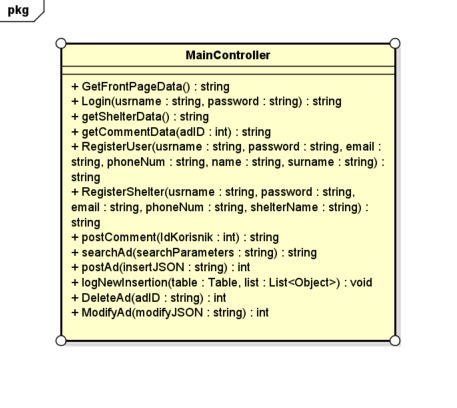
\includegraphics[scale =0.4]{kontroler.JPEG}
				\centering
				\caption{Dijagram razreda - dio Controllers}
				\label{fig:your_label}
			\end{figure}
			
			\begin{figure}[H]
				
				\includegraphics[scale =0.4]{model.JPEG}
				\centering
				\caption{Dijagram razreda - dio Models}
				\label{fig:your_label}
			\end{figure}
			%\eject
		
		\section{Dijagram stanja}
			
			
			%\textbf{\textit{dio 2. revizije}}\\
			
			%\textit{Potrebno je priložiti dijagram stanja i opisati ga. Dovoljan je jedan dijagram stanja koji prikazuje \textbf{značajan dio funkcionalnosti} sustava. Na primjer, stanja korisničkog sučelja i tijek korištenja neke ključne funkcionalnosti jesu značajan dio sustava, a registracija i prijava nisu. }
			
			Dijagram stanja strukturirano prikazuje kako sustav ili njegovi dijelovi prelaze iz jednog stanja u drugo kao odgovor na neki događaj. Na slici (broj) prikazan je dijagram stanja za registriranog korisnika. Nakon prijave u sustav, korisniku se prikazuje početna stranica na kojoj je vidljiva lista oglasa. Odabirom oglasa, prikazuju se podaci o izgubljenom kućnom ljubimcu. Korisnik ima mogućnost ostaviti komentar na oglasu ukoliko ima informaciju koja bi mogla pomoći u potrazi za izgubljenom životinjom. Korisnik može odabrati neku od mogućnosti iz navigacijske trake. Odabirom na „Neaktivni oglasi“, prikazuju se oglasi svih kategorija, osim one da se za ljubimcem aktivno traga. Klikom na „Skloništa“, prikazuje se lista skloništa, a odabirom na neko od skloništa prikazuju se podaci o skloništu te oglasi od odabranog skloništa, ako ih ima. Klikom na korisničko ime, prikazuju se oglasi korisnika, koje korisnik može urediti ili izbrisati. Također, korisnik ima mogućnost stvaranja novog oglasa.
			
			\begin{figure}[H]
				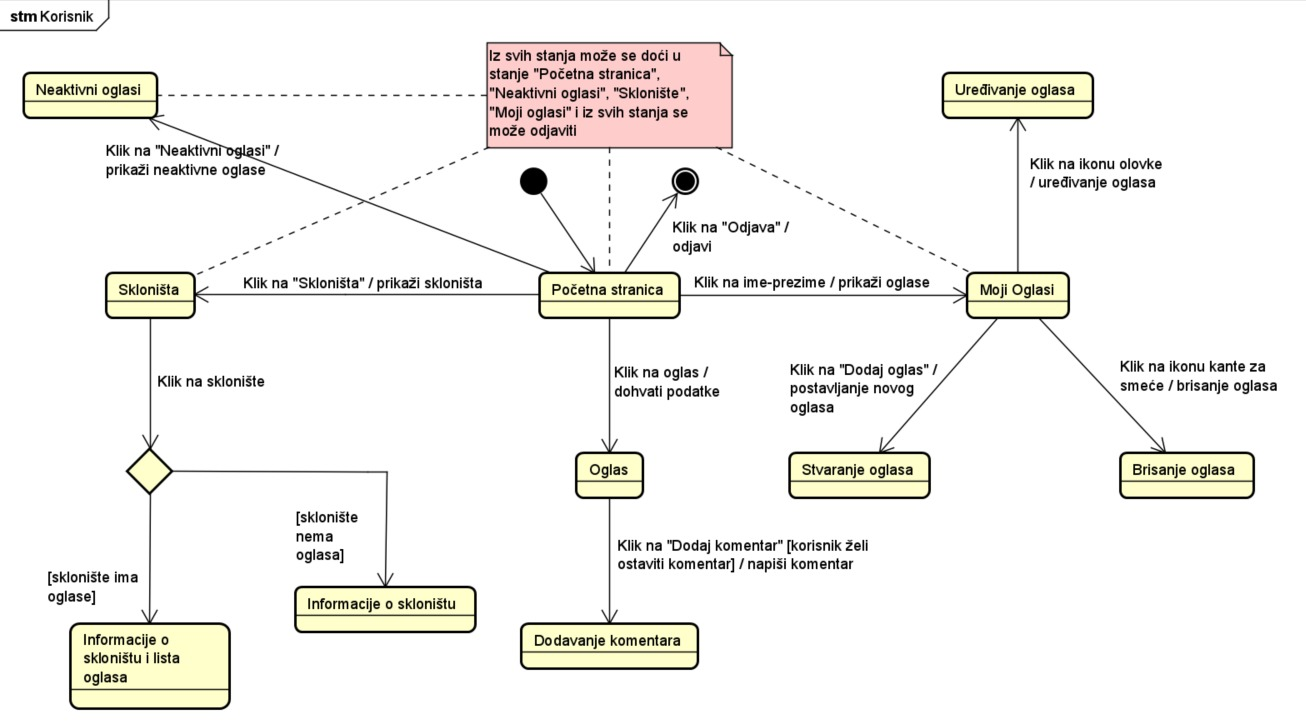
\includegraphics[width=\textwidth]{dijagram_stanja.JPEG}
				\centering
				\caption{Dijagram stanja - registrirani korisnik}
				\label{fig:dijagramstanja}
			\end{figure}
			
			
			\eject 
		
		\section{Dijagram aktivnosti}
			
			\textbf{\textit{dio 2. revizije}}\\
			
			 \textit{Potrebno je priložiti dijagram aktivnosti s pripadajućim opisom. Dijagram aktivnosti treba prikazivati značajan dio sustava.}
			
			\eject
		\section{Dijagram komponenti}
		
			\textbf{\textit{dio 2. revizije}}\\
		
			 \textit{Potrebno je priložiti dijagram komponenti s pripadajućim opisom. Dijagram komponenti treba prikazivati strukturu cijele aplikacije.}